\section{Flow Network}

\subsection{Definitions}

We can interpret a graph as a ``flow network'' and use it to model the flow of materials such as water through pipes, electricity through wires, or goods through supply chain. Each flow network will have a source where everything originates from and a sink (destination) where everything arrives at. We first formally define a \textit{\textbf{flow network}}.

\begin{definition}[Flow Network] \index{flow network} \index{source} \index{sink}
    A \textit{\textbf{flow network}} $G=(V,E)$ is a directed network in which each edge $(u,v) \in E$ has a nonnegative capacity $c(u,v) \geq 0$. Additionally, if $(u,v) \in E$, then $(v,u) \not\in E$. If $(u,v) \not\in E$, then $c(u,v) = 0$.

    In particular, in a flow network, there is a \textit{\textbf{source}} $s$ and \textit{\textbf{sink}} $t$, and every vertex lies on some path from from $s$ to $t$. That is, $\forall v \in V$, there exists a path $p$ such that $p = s \leadsto v \leadsto t$.
\end{definition}

\begin{definition}[Flow] \index{flow}
    Let $G=(V,E)$ be a flow network with capacity function $c:\, V\times V \to \R$, and let $s$ be the source and $t$ be the sink of the network. A \textit{\textbf{flow}} in $G$ is a function $f:\, V\times V \to \R$ that satisfies the following properties:
    \begin{itemize}
        \item Capacity constraint: for all $u,v \in V$, $0 \leq f(u,v) \leq c(u,v)$.
        \item Flow conservation: for all $u \in V - \{s,t\}$, $\sum_{v \in V} f(v,u) = \sum_{v \in V} f(u,v)$. That is, the flow into $u$ must equal the flow out from $u$. When $(u,v) \not\in E$, $f(u,v) = 0$.
    \end{itemize}
    We define the \textit{\textbf{value}} of a flow $f$ to be
    $$
    |f| = \sum_{v\in V} f(s,v) - \sum_{v \in V} f(v,s)
    $$
    Sometimes, we abuse notations a little bit and omit the summation by writing $f(s,V)$ where $V$ is the set of vertices. Some also uses the notation $f_{in}(v)$ and $f_{out}(v)$ to denote the flow into and out from $v$, respectively.
\end{definition}

\begin{example}[Example of a Flow Network]
    Below is an example of flow network. On each edge $(u,v) \in E$, we write $f(u,v) / c(u,v)$. The slash is simply a separator and does not mean division.

\end{example}

The goal of the maximum flow problem is to find a flow $f$ that maximizes the value of the flow $|f|$. This is also equivalent to finding the maximum flow into the sink $t$.

The max-flow problem is interesting not only because its practical applications, but also its relation to other problems. Many other problems are closely related to the max-flow problem can be polynomial-time reduced to the max-flow problem.

\subsection{Antiparallel Edges and Multiple Sources/Sinks}

In our definition of a flow network, we requires there to be exactly only one source and one sink, and we prohibit antiparallel edges (i.e. if $(u,v) \in E$, then $(v,u) \not\in E$).

However, it is easy to convert a graph with multiple sources and/or sinks and antiparallel edges into a flow network that fit our original definition.

\begin{theorem}
    Suppose that a graph $G$ contains an edge $(u,v)$. We can create a new flow network $G'=(V',E')$ where $V' = V \cup \{x\}$ and $E' = E - \{(u,v)\} \cup \{(u,x),(x,v)\}$. $G'$ is obtained by creating a new vertex $x$ and replacing $(u,v)$ by $(u,x),(v,x)$. We set the capacity $c(u,x) = c(x,v) = c(u,v)$. The maximum flow in $G'$ is the same as the maximum flow in $G$.
\end{theorem}

\begin{proof}
    
\end{proof}

\begin{theorem}
    Let $G$ be a graph with multiple source vertices and multiple sink verticies. Let $G'$ be constructed as follows. Suppose $G$ has sources $S=\{s_1,\ldots,s_i\}$ and sinks $T=\{t_1,\ldots,t_j\}$. We add a supersource $s$ and edges $(s,s_i)$ with capacity $c(s,s_i) = \infty$ for all $s_i \in S$. We add a supersink $t$ and edges $(t_j,t)$ for all $t_j \in T$ with capacity $c(t_j,t) = \infty$. More formally, $G'=(V',E')$ such that $V' = V \cup \{s\} \cup \{t\}$ and $E' = E \cup \{(s,s_i) \mid s_i \in S\} \cup \{(t_j,t) \mid t_j \in T\}$. $G'$ has the same maximum flow as $G$.
\end{theorem}

\begin{proof}
    
\end{proof}

This theorem will become useful later when we look at the maximum bipartite matching problem.

\section{Ford-Fulkerson Method} \index{Ford-Fulkerson method}

\textit{\textbf{Ford-Fulkerson method}} is a general approach to solve the maximum flow problem. It uses an incremental improve approach by gradually increasing the flow until we reach the maximum. More generally, Ford-Fulkerson can be viewed as a greedy local search algorithm. It is called a method or a scheme because most parts of it can be implemented differently but the general approach remains the same.

The table below summarizes some of the common implementation of the Ford-Fulkerson method. At the end of this chapter, we will discuss the Edmonds-Karp algorithm, and in a later chapter, we will discuss a different algorithm known as the push-relabel algorithm, which uses a different approach than Ford-Fulkerson.

\begin{table}[htpb]
    \centering
    \begin{tabular}{c|c|c}
    Algorithm & Implementation & Complexity \\
    \hline
    Edmonds-Karp (1970) & BFS for finding augmenting path & $O(|E|^2|V|)$ \\
    Dinitz (1970) & BFS + DFS for finding augmenting path & $O(|V|^2 |E|)$ \\
    Capacity Scaling (Dinitz, 1972) & Capacity scaling heuristic & $O(|E|^2 \log c_{max})$ \\
    Dinitz-Gabow (1973) & Capacity scaling heuristic & $O(|V||E| \log c_{max})$ 
    \end{tabular}
    \caption{Comparison of multiple algorithms based on the Ford-Fulkerson. $c_{max}$ in capacity scaling denotes the largest capacity in the network.}
    \label{tab:ford-fulkerson}
\end{table}

\subsection{Idea Behind Ford-Fulkerson}

The idea behind Ford-Fulkerson is quite simple. For each iteration of the algorithm, we find a path from $s$ to $t$, increase the flow along the path until we hit a bottleneck at one of the edges on the path (the edge with the smallest remaining capacity). This is called augmenting flow, and the path is called augmenting path. When augmenting the flow along the augmenting path, we may also want to decrease the flow along each residue (i.e. reverse) edge so that we can ``undo'' bad augmentation choices. We will show that when the algorithm terminates, it correctly returns the max-flow.

Note that this is more precisely, only the partial correctness. Surprisingly, depending on the implementation and capacities, the algorithm may not terminate. In particular, the Ford-Fulkerson method may fail to terminate if edge capacities are irrational \cite{Zwick-FF-Example}. In his 1993 paper, Zwick showed a minimal example flow network (with 6 vertices and 8 edges) on which Ford-Fulkerson fails to terminate.

\begin{codebox}
    \Procname{$\proc{Ford-Fulkerson}(G,s,t)$}
    \li $f = 0$ for all $(u,v) \in E$ 
    \li \While there exists an augmenting path $p$ in residue network $G_f$ \Do
        \li augment flow $f$ along $p$
    \End
    \li \Return $f$
\end{codebox}

\section{Correctness of Ford-Fulkerson}

\subsection{Residue Network and Augmentation}

Let us make the idea more concrete by formalizing it and proving the correctness of the Ford-Fulkerson method. We first define what a residue network is.

Given a flow network $G$, the residue network $G_f$ contains edges with capacities that represent how much more flow we can push through each edge. For each edge $(u,v)$, we will also add backward edges $(v,u)$ to the residue network that can at most cancel out the flow through the edge $(u,v)$.

\begin{definition}[Residue Capacity] \index{residue capacity}
    Let $G=(V,E)$ be a flow network with source $s$ and sink $t$. Let $f$ be a flow in $G$, and consider a pair of vertices $u,v \in V$. The \textit{\textbf{residue capacity}} $c_f(u,v)$ is defined as
    $$
    c_f(u,v) = \begin{cases}
        c(u,v) - f(u,v) & (u,v) \in E \\
        f(v,u) & (v,u) \in E \\
        0 & \text{otherwise}
    \end{cases}
    $$
    By assumption, since $G$ is a flow network, $(u,v) \in E \iff (v,u) \not\in E$, exactly one case in the definition applies.
\end{definition}

\begin{definition}[Residue Network] \index{residue network}
    Let $G=(V,E)$ be a flow network and a flow $f$. The \textit{\textbf{residue network}} of $G$ induced by $f$, denoted $G_f$ is $G_f = (V,E_f)$ where $E_f = \{(u,v) \in V \times V \mid c_f(u,v) > 0 \}$.
\end{definition}
A residue network contains at most twice many edges as the original flow network. If an edge does not exist in $G$ (has zero capacity), it does not exist in $G_f$ either.

\begin{definition}[Augmentation] \index{augmentation (max-flow)}
    Let $G=(V,E)$ be a flow network with flow $f$. $G_f$ is the residue network of $G$ induced by $f$. Suppose that $f'$ is a flow in $G_f$. We define the \textit{\textbf{augmentation}} of $f$ by $f'$, denoted $f \uparrow f'$, to be a function $(f \uparrow f'):\, V\times V \to \R$ such that
    $$
    (f \uparrow f')(u,v) = \begin{cases}
        f(u,v) + f'(u,v) - f'(v,u) & (u,v) \in E \\
        0 & \text{otherwise}
    \end{cases}
    $$
\end{definition}

Note that because we allow backward edges in a residue network, we need to subtract $f'(v,u)$ when augmenting $f$ and $f'$ on edge $(u,v)$. The notion of pushing flow through a reverse edge is called cancellation.

\begin{lemma} \label{lem:value-of-augmented-flow}
    Let $G=(V,E)$ be a flow network with source $s$ and sink $t$, and let $f$ be a flow in $G$. Let $G_f$ be the residue network of $G$ induced by $f$, and let $f'$ be a flow in $G_f$. Then $f \uparrow f'$ is a flow in $G$ and $|f \uparrow f'| = |f| + |f'|$.
\end{lemma}

\begin{proof}
    To show that $f \uparrow f'$ is a flow in $G$, it suffices to show the capacity constraint and flow conservation properties hold.

    Capacity constraint: Let $u,v \in V$. Then, \\ $(f \uparrow f')(u,v)=f(u,v)+f'(u,v)-f'(v,u) \leq f(u,v) + f'(u,v) \leq f(u,v) + c_f(u,v) = f(u,v) + c(u,v) - f(u,v) = c(u,v)$.

    Flow conservation: Fix $u \in V$. Let $In(u) = \{v \in V \mid (u,v) \in E\}$ and $Out(u) = \{v \in V \mid (u,v) \in E\}$. That is, $In(u)$ is the set of vertices with edges to $u$ and $Out(u)$ is the set of vertices with edges from $u$.
    $$
    \begin{aligned}
        \sum_{v \in Out(u)} (f \uparrow f')(u,v) - \sum_{v \in In(u)} (f \uparrow f')(v,u) =&
        \sum_{v \in Out(u)} f(u,v) + \sum_{v \in Out(u)} f'(u,v) - \sum_{v \in Out(u)} f'(v,u) - \\
        & \sum_{v \in In(u)} f(v,u) - \sum_{v \in In(u)} f'(v,u) + \sum_{v \in In(u)} f'(u,v)
    \end{aligned}
    $$
    Regrouping the terms yields \\ $\sum_{v \in Out(u)} f(u,v) - \sum_{v \in In(u)} f(v,u) + [\sum_{v \in Out(u)} f'(u,v) + \sum_{v \in In(u)} f'(u,v) ] \\ - [ \sum_{v \in Out(u)} f'(v,u) + \sum_{v \in In(u)} f'(v,u) ]$,
    
    which is equivalent to $\sum_{v \in V} f(u,v) - \sum_{v \in V} f(v,u) + \sum_{v \in V} f'(u,v) - \sum_{v \in V} f'(v,u)$. We can extend the summation from $In(u)$ and $Out(u)$ to $V$ because all the additional terms are 0 by definition of flow and the fact that there $(u,v) \not\in E$ for $v \in V-Out(u)$ and $(v,u) \not\in E$ for $v \in V-In(u)$.

    By flow conservation of $f$ and $f'$ individually, \\
    $\sum_{v \in V} f(u,v) - \sum_{v \in V} f(v,u) + \sum_{v \in V} f'(u,v) - \sum_{v \in V} f'(v,u) = 0$, \\
    which implies that $\sum_{v \in Out(u)} (f \uparrow f')(u,v) = \sum_{v \in In(u)} (f \uparrow f')(u,v)$.

    To show that $|f \uparrow f'| = |f| + |f'|$, set $u = s$ in the previous derivation, and we have
    $$
    \begin{aligned}
        |f \uparrow f'| &= \sum_{v \in Out(s)} (f \uparrow f')(s,v) - \sum_{v \in In(s)} (f \uparrow f')(v,s) \\
        &= \sum_{v \in V} f(s,v) - \sum_{v \in V} f(v,s) + \sum_{v \in V} f'(s,v) - \sum_{v \in V} f'(v,s) \\
        &= |f| + |f'|.
    \end{aligned}
    $$
\end{proof}

\subsection{Augmenting Paths}

\vspace{\parskip}

\begin{definition}[Augmenting Path] \index{augmenting path}
    Given a flow network $G=(V,E)$ with source $s$ and sink $t$ and flow $f$, an \textit{\textbf{augmenting path}} $p$ is a simple path from $s$ to $t$ in the residue graph $G_f$ of $G$ induced by $f$.
\end{definition}

\begin{definition}[Residue Capacity of an Augmenting Path]
    Let $p$ be an augmenting path for the flow network $G$. Then, the \textit{\textbf{residue capacity}} of $p$ is defined as the maximum amount by which we can increase the flow on each edge in the $p$, or more formally,
    $$
    c_f(p) = \min \{c_f(u,v) \mid \text{$(u,v)$ is on $p$} \}
    $$
\end{definition}

\begin{definition}[Flow of an Augmenting Path]
    Let $G=(V,E)$ be a flow network, $f$ be a flow in $G$, and let $p$ be an augmenting path in $G_f$. Define the flow of the augmenting path $f_p:\, V \times V \to \R$ by
    $$
    f_p(u,v) = \begin{cases}
        c_f(p) & \text{$(u,v)$ on $p$} \\
        0 & \text{otherwise}
    \end{cases}
    $$
\end{definition}

\begin{lemma} \label{lem:augmenting-flow}
    The flow $f_p$ on an augmenting path $p$ is a flow in $G_f$ with value $|f_p| = c_f(p) > 0$.
\end{lemma}

\begin{proof}
    We show that $f_p$ satisfies the capacity constraint and flow conservation.

    Capacity constraint: If $(u,v)$ is on $p$, then $f_p(u,v)=c_f(p) \leq c_f(u,v)$ by definition. If $(u,v)$ is not on $p$, then $f_p(u,v) = 0 \leq c_f(p)$.

    Flow conservation: Fix $u \in V - \{s,t\}$. First, consider the case where $u$ is on $p$. Say, edges $(w,u)$ and $(u,v)$ are on $p$. Then, since $p$ is a simple path and $u \in V-\{s,t\}$, there is exactly one edge going into and out from $u$. $\sum_{v \in In(u)} f_p(v,u) = f_p(w,u) = c_f(p)$ and $\sum_{v \in Out(u) f_p(u,v)} = f_p(u,v) = c_f(p)$. If $(u,v)$ is not on $p$, both the flow into $u$ and flow out from $u$ are 0. In both cases, flow conservation is satisfied.

    Finally, to show that $|f_p| = c_f(p)$, consider the flow out from $s$. Since $p$ is a simple path, there is no flow input $s$, so $|f_p| = \sum_{v \in V} f(s,v) - \sum_{v \in V} f(v,s) = c_f(p) - 0 = c_f(p)$ 
\end{proof}

Immediately following from Lemma \ref{lem:augmenting-flow} and \ref{lem:value-of-augmented-flow}, we have the following corollary.

\begin{corollary} \label{corollary:augmentation-increases-flow}
    Let $G=(V,E)$ be a flow network, let $f$ be a flow in $G$, and let $p$ be an augmenting path in $G_f$. Let $f_p$ be a flow on the augmenting path defined previously. Then, $f \uparrow f_p$ is a flow in $G$ with value
    $$
    |f \uparrow f_p| = |f| + |f_p| > |f|
    $$
\end{corollary}

\begin{proof}
    By Lemma \ref{lem:value-of-augmented-flow}, $|f_p| = c_f(p) > 0$. By Lemma \ref{lem:augmenting-flow}, $f \uparrow f_p$ is a flow and has value $|f|+|f_p| > |f|$.
\end{proof}

As a result of Corollary \ref{corollary:augmentation-increases-flow}, we know that augmenting a flow with an augmenting path yields a flow with value strictly greater than the flow prior to augmentation.

\subsection{Max-Flow Min-Cut Theorem}

Our analyses so far shows a promising picture of the correctness of the Ford-Fulkerson method. By iteratively augmenting $f$ with an augmenting path $p$, we gradually increases the flow in the flow network, and when the procedure halts, we should expect to see that $f$ is equal to the maximum flow. The proof utilizes the max-flow min-cut theorem and shows that if there is no augmenting path, there exists a cut in the flow network that implies that $f$ is the max-flow.

\begin{definition}[Cut and Net Flow Across a Cut] \index{cut} \index{minimum cut}
    A \textit{\textbf{cut}} $(S,T)$ of flow network $G=(V,E)$ is a partition of $V$ into $S$ and $T=V-S$ such that $s \in S$ and $t \in T$. If $f$ is a flow, then the \textit{\textbf{net flow}} $f(S,T)$ across the cut $(S,T)$ is defined as
    $$
    f(S,T) = \sum_{u \in S}\sum_{v \in T} f(u,v) - \sum_{u \in S}\sum_{v \in T} f(v,u)
    $$
    The \textit{\textbf{capacity of the cut}}, denoted $c(S,T)$ is
    $$
    c(S,T) = \sum_{u \in S}\sum_{v \in T} c(u,v)
    $$
\end{definition}
A \textit{\textbf{minimum cut}} is a cut whose capacity is minimum over all cuts of the flow network. The definition of a cut and minimum cut will help us prove the important max-flow min-cut theorem. The proof roughly follows the outline shown in Figure \ref{fig:maxflow-ford-fulkerson-proof}.

\begin{figure}[htbp]
    \centering
    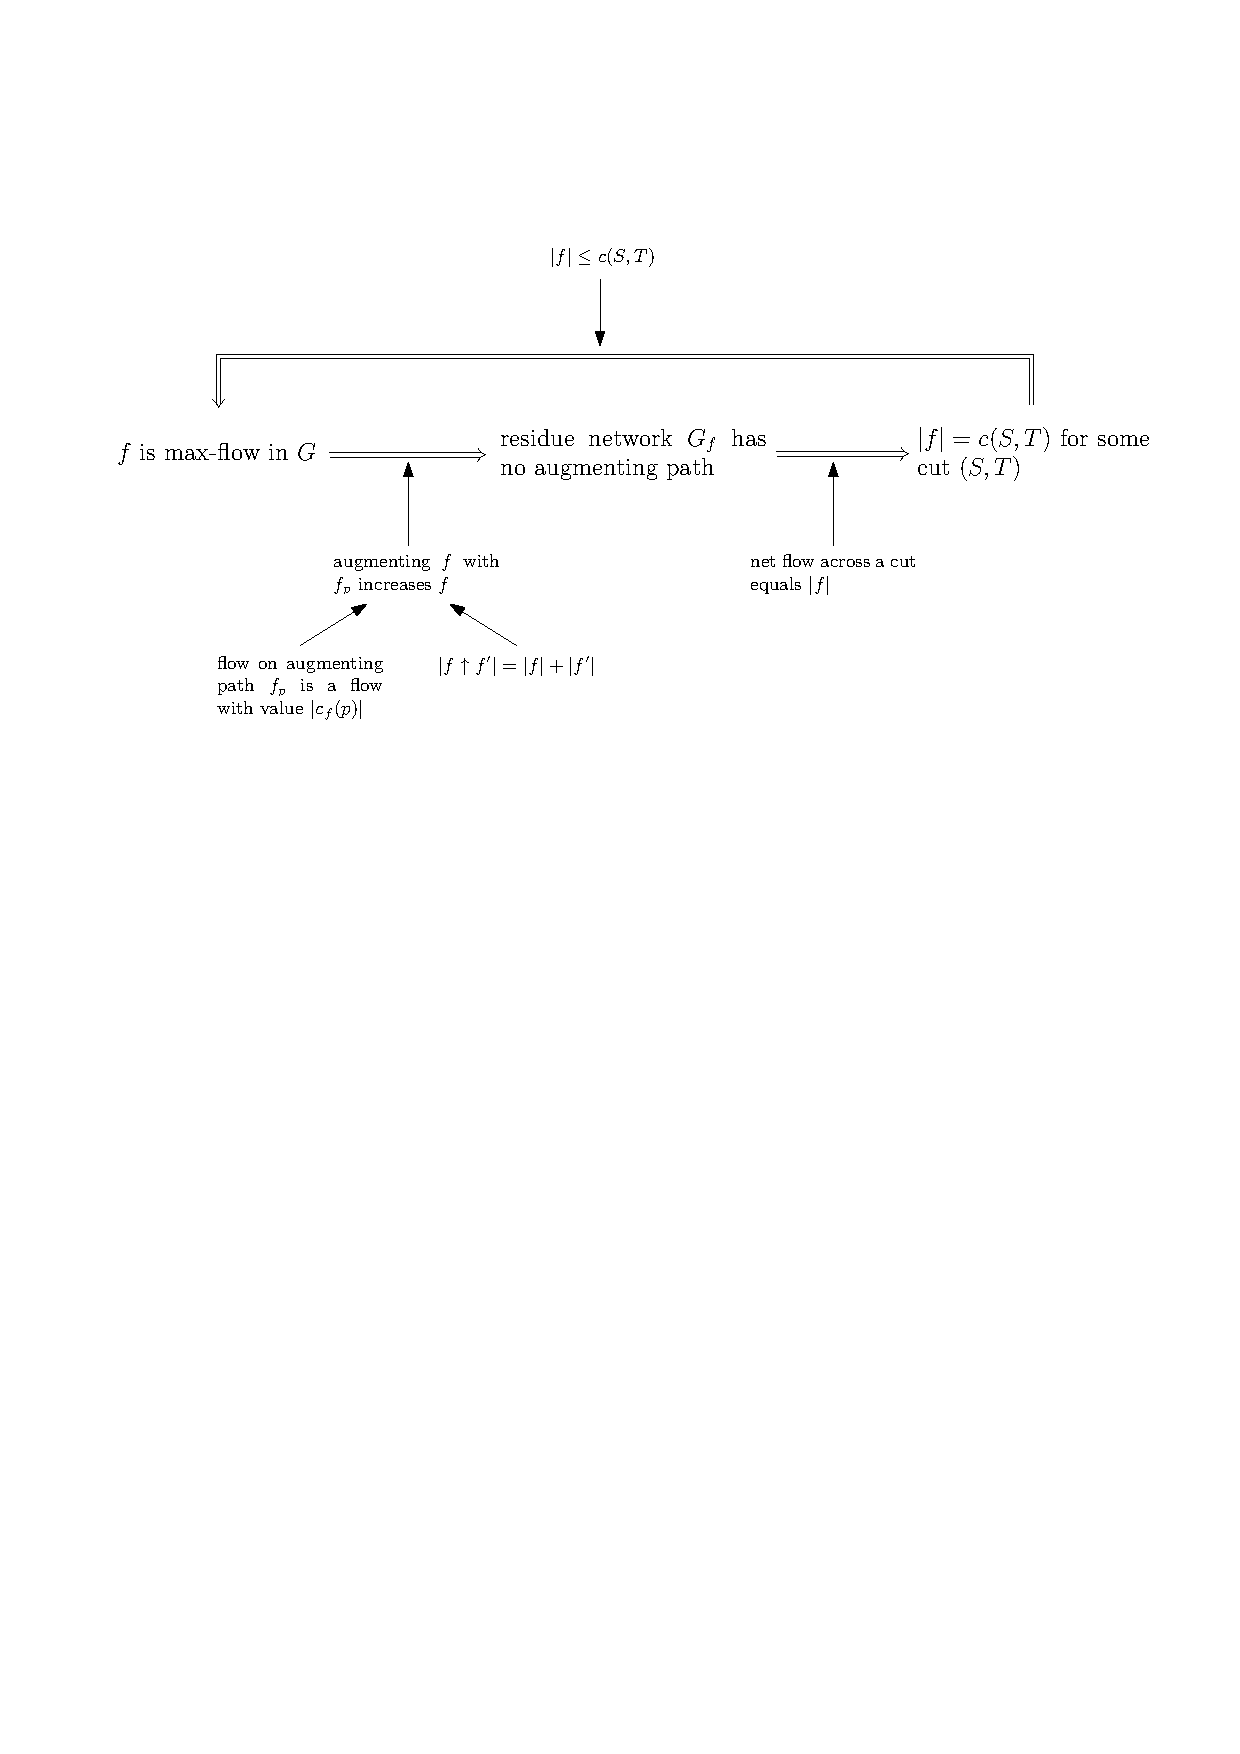
\includegraphics[width=0.95\linewidth]{maxflow/maxflow-mincut-proof-outline.pdf}
    \hfill
    \caption{Proof outline for the partial correctness of the Ford-Fulkerson method.}
    \label{fig:maxflow-ford-fulkerson-proof}
\end{figure}

\begin{lemma} \label{lem:flow-across-cut}
    Let $f$ be a flow in a flow network $G$ with source $s$ and sink $t$. Let $(S,T)$ be a cut of $G$. Then, the net flow across the cut $(S,T)$ is $f(S,T) = |f|$.
\end{lemma}

\begin{proof}
    Let $(S,T)$ be a cut in $G$. Consider the following net flows:
    \begin{itemize}
        \item $f(S,T)$: the net flow across the cut $(S,T)$ 
        \item $f(S,V)$: the net flow for edges starting in $S$
        \item $f(S,S)$: the net flow within $S$ 
        \item $f(\{s\},V)$: the net flow from $s$ (i.e. $|f|$)
        \item $f(S-\{s\},V)$: the net flow of edges that start from the partition $S$ but not the source $s$ 
    \end{itemize}
    Fix $u \in V - \{s,t\}$. By flow conservation, we have $\sum_{v \in V} f(u,v) - \sum_{v \in V} f(v,u) = 0$. This is true for all $u \in V - \{s,t\}$, so 
    $$\sum_{u \in S-\{s\}} \left(\sum_{v \in V} f(u,v) - \sum_{v \in V} f(v,u)\right) = 0.$$ 
    
    This summation can be expanded to 
    $$\sum_{u \in S-\{s\}}\sum_{v \in V} f(u,v) - \sum_{u \in S-\{s\}}\sum_{v \in V} f(v,u) = 0$$
    by linearity. Note this expression is equivalent to $f(S-\{s\},V)$ by definition. So, $f(S-\{s\},V) = 0$.

    Now consider $f(S,S)$. By definition, we can rewrite $f(S,S)$ as 
    $$\sum_{u \in S}\sum_{v \in S} f(u,v) - \sum_{u \in S}\sum_{v \in S} f(v,u) = 0$$
    because for all vertices $x,y \in S$, the term $f(x,y)$ appears exactly once in each summation. Hence, $f(S,S) = 0$.

    Since $V = S \cup T$ and $S \cap T = \emptyset$,
    $$
    \begin{aligned}
        f(S,T) &= f(S,V) - f(S,S) \\
        &= f(S,V) \\
        &= f(\{s\},V) + f(S-\{s\},V) \\
        &= f(\{s\},V) \\
        &= |f|
    \end{aligned}
    $$ 
\end{proof}
This proof is inspired by the proof presented in the second edition of CLRS. The proof in the third edition employs a more rigorous argument using properties of summation, but I personally find it less intuitive.

A corollary to this lemma shows that cut capacity can be used to bound the value of a flow.

\begin{corollary} \label{corollary:flow-upper-bound}
    The value of any flow $f$ in a flow network $G$ is bounded above by the capacity of any cut of $G$.
\end{corollary}

\begin{proof}
    Let $(S,T)$ be a cut of $G$ and let $f$ be a flow. By Lemma \ref{lem:flow-across-cut} and capacity constraint,
    $$
    \begin{aligned}
        |f| = f(S,T) &= \sum_{u \in S}\sum_{v \in T}f(u,v) - \sum_{u \in S}\sum_{v \in T}f(v,u) \\
        &\leq \sum_{u \in S}\sum_{v \in T}f(u,v) \\
        &\leq \sum_{u \in S}\sum_{v \in T} c(u,v) & \text{capacity constraint} \\
        &= c(S,T) & \text{definition}
    \end{aligned}
    $$
\end{proof}

Now we finally have everything we need to prove the max-flow min-cut theorem. We will follow the proof outline to prove the equivalences (iff).

\begin{theorem}[Max-Flow Min-Cut Theorem] \index{max-flow min-cut theorem}
    If $f$ is a flow in a flow network $G=(V,E)$ with source $s$ and sink $t$, then the following conditions are equivalent
    \begin{enumerate}
        \item $f$ is a maximum flow in $G$ 
        \item The residue network $G_f$ contains no augmenting paths
        \item $|f| = c(S,T)$ for some cut $(S,T)$ of $G$ 
    \end{enumerate}
\end{theorem}

\begin{proof}
    \hfill

    (1) $\Rightarrow$ (2): Suppose, for contradiction, that $f$ is a maximum flow in $G$, but $G_f$ has a new augmenting path $p$. Then, by Corollary \ref{corollary:augmentation-increases-flow}, the flow obtained by augmenting $f$ and $f_p$ has a strictly greater value and $f \uparrow f_p$ is a flow in $G$. This contradicts the assumption that $f$ is a maximum flow. 

    (2) $\Rightarrow$ (3): Assume (2) holds. Then, there is no path from $s$ to $t$ in the residue network $G_f$. Let $S = \{ u \in V \mid \text{there exists a path from $s$ to $u$ in $G_f$} \}$, and let $T = V-S$. Clearly, $(S,T)$ is a cut (this can be trivially proved by showing $s \in S$ and $t \not\in S$ because there is no path from $s$ to $t$). We claim that for each $u\in S$ and $v \in T$, $(u,v) \in E$, $f(u,v) = c(u,v)$. To see why this is true, we use proof by contradiction. Suppose the claim is false. By capacity constraint $f(u,v) \leq c(u,v)$. If $f(u,v) \neq c(u,v)$, $f(u,v) < c(u,v)$ and $(u,v) \in E_f$ because it would have positive residue capacity. But then, this means there would be a path from $u$ to $v$ and $v \in S$, contradicting the assumption that $v \in T$. The other case where $(v,u) \in E$ follows from the same argument with $u$ and $v$ swapped.

    (3) $\Rightarrow$ (1): Assume (3) holds. Then, there exists a cut $(S,T)$ such that $|f| = c(S,T)$. By Corollary \ref{corollary:flow-upper-bound}, $|f| \leq c(S,T)$. This implies that every other flow has value less than $f$, so $f$ is a maximum flow.
\end{proof}

This theorem shows that if Ford-Fulkerson terminates, then the resulting flow is the maximum flow. The proof of correctness also suggests the following algorithm that elaborates on the Ford-Fulkerson method outline described earlier.

\begin{codebox}
    \Procname{$\proc{Ford-Fulkerson}(G=(V,E),s,t)$}
    \li \For each $(u,v) \in E$ \Do
        \li $(u,v).f = 0$ \RComment{initialize flow to 0}
    \End
    \li \While there exists a path $p$ from $s$ to $t$ in the residue network $G_f$ \Do
        \li $c_f(p) = \min \{c_f(u,v) \mid \text{$(u,v)$ is on $p$} \}$ \RComment{residue capacity of path $p$}
        \li \For each $(u,v)$ on $p$ \Do \RComment{augment flow}
            \li \If $(u,v) \in E$ \Then
                \li $(u,v).f = (u,v).f + c_f(p)$
            \li \Else $(v,u).f = (v,u).f - c_f(p)$
            \End
        \End
    \End
\end{codebox}

This gives us an upper bound on the running time of the Ford-Fulkerson method. Without loss of generality, we can assume that the capacities are integral (otherwise we can rescale them to integers). Then, we know that each iteration of the while loop increases the flow value by at least one unit. Hence, the while loop of Line 3-8 runs at most $|f^*|$ iterations where $f^*$ is the maximum flow. We can find the augmenting path $p$ using either BFS or DFS, which can be done in $O(|E|)$ time. Since we need to find an augmenting path for every iteration of the while loop and the while loop runs at most $|f^*|$ iterations, we can conclude that the running time of the Ford-Fulkerson method is upper bounded by $O(|f^*||E|)$. 

A better upper bound on the running time of Ford-Fulkerson's algorithm/method depends on the way we implement the procedure for finding augmenting path $p$. In the next chapter, we will look at Edmonds-Karp's algorithm, which implements this operation using BFS.

\section{Irrational Capacity}

The Ford-Fulkerson method may fail to terminate on a flow network with irrational capacities. We will present an example of such network, first discovered by Zwick in 1993 \cite{Zwick-FF-Example}.

\begin{figure}[htbp]
    \centering
    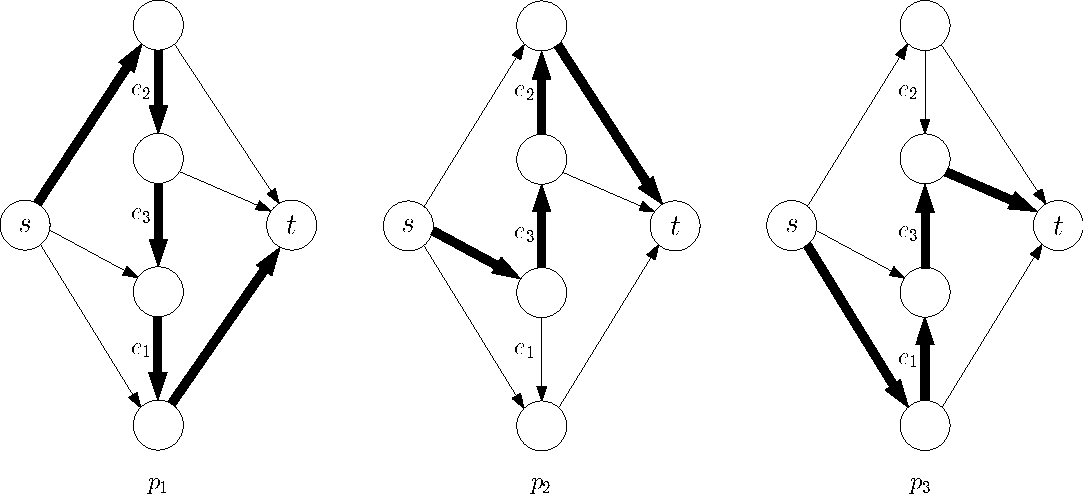
\includegraphics[width=0.8\linewidth]{maxflow/ff-counterexample.pdf}
    \caption{3 augmenting paths for the nonterminating example}
    \label{fig:ff-counterexample-augment-path}
\end{figure}